\section{Elementos clave del tablero Kanban}

El tablero Kanban es la herramienta visual central de esta metodología. A través de él se representa gráficamente el flujo de trabajo de un equipo, permitiendo monitorear el estado de las tareas, identificar cuellos de botella y tomar decisiones informadas para mejorar el rendimiento del sistema. Un tablero bien diseñado refuerza la transparencia, la colaboración y la responsabilidad compartida.

\subsection{Columnas del tablero}

Las columnas representan los distintos estados o fases que atraviesa una tarea desde su inicio hasta su finalización. Aunque la estructura más común es la de tres columnas —``Por hacer'' (\textit{To Do}), ``En progreso'' (\textit{Doing}) y ``Hecho'' (\textit{Done})—, el tablero puede adaptarse a las particularidades del proceso específico de cada equipo. Algunas configuraciones incluyen columnas como:
\begin{itemize}
    \item \textbf{Análisis / Diseño}
    \item \textbf{Desarrollo}
    \item \textbf{Pruebas / Revisión}
    \item \textbf{Aprobación del cliente}
\end{itemize}

La clave es que cada columna represente claramente una etapa del flujo de trabajo.

\subsection{Tarjetas de tareas}

Las tarjetas o fichas son unidades visuales que representan elementos de trabajo concretos (por ejemplo, una funcionalidad, una corrección o un documento). Estas tarjetas contienen información clave como:
\begin{itemize}
    \item Título y descripción de la tarea
    \item Responsable asignado
    \item Prioridad o etiqueta (urgente, bloqueado, etc.)
    \item Fecha de inicio y estimación de finalización
\end{itemize}

El movimiento de las tarjetas entre columnas refleja el avance del trabajo. Además, su diseño puede personalizarse para incorporar colores, íconos o códigos que ayuden a su rápida interpretación.

\subsection{Swimlanes o carriles horizontales}

Los \textit{swimlanes} permiten segmentar el tablero horizontalmente, organizando las tareas por tipo, proyecto, equipo o prioridad. Por ejemplo, en un equipo multifuncional, se pueden utilizar carriles como:
\begin{itemize}
    \item Funcionalidades nuevas
    \item Corrección de errores
    \item Mantenimiento técnico
\end{itemize}

Este recurso mejora la claridad del tablero cuando se gestionan múltiples flujos paralelos o categorías de trabajo distintas.

\subsection{Límites de trabajo en curso (WIP)}

El tablero Kanban incluye indicadores de \textit{Work In Progress} que limitan la cantidad de tareas permitidas por columna. Estos límites se indican explícitamente en el encabezado de cada columna (por ejemplo, ``En progreso (máx. 3)''). Esta restricción busca:
\begin{itemize}
    \item Reducir el trabajo multitarea
    \item Prevenir la acumulación excesiva
    \item Favorecer la finalización de tareas antes de iniciar nuevas
\end{itemize}

El cumplimiento de los límites WIP es clave para mantener la eficiencia del sistema y evitar bloqueos.

\subsection{Indicadores visuales adicionales}

Además de columnas, tarjetas y límites WIP, los tableros Kanban pueden incorporar elementos visuales complementarios como:
\begin{itemize}
    \item \textbf{Etiquetas de colores}: para marcar prioridades o categorías
    \item \textbf{Íconos}: para señalar tareas bloqueadas, pendientes de revisión o requerimientos especiales
    \item \textbf{Checklist}: para tareas con subtareas internas
    \item \textbf{Diagramas de flujo acumulativo}: para analizar tendencias de rendimiento
\end{itemize}

Estos recursos aumentan la capacidad de análisis del tablero y mejoran la toma de decisiones en tiempo real.

\subsection{Ejemplo visual de un tablero Kanban}

A continuación se presenta un ejemplo simplificado de un tablero Kanban con sus principales componentes:

\begin{figure}[H]
\centering
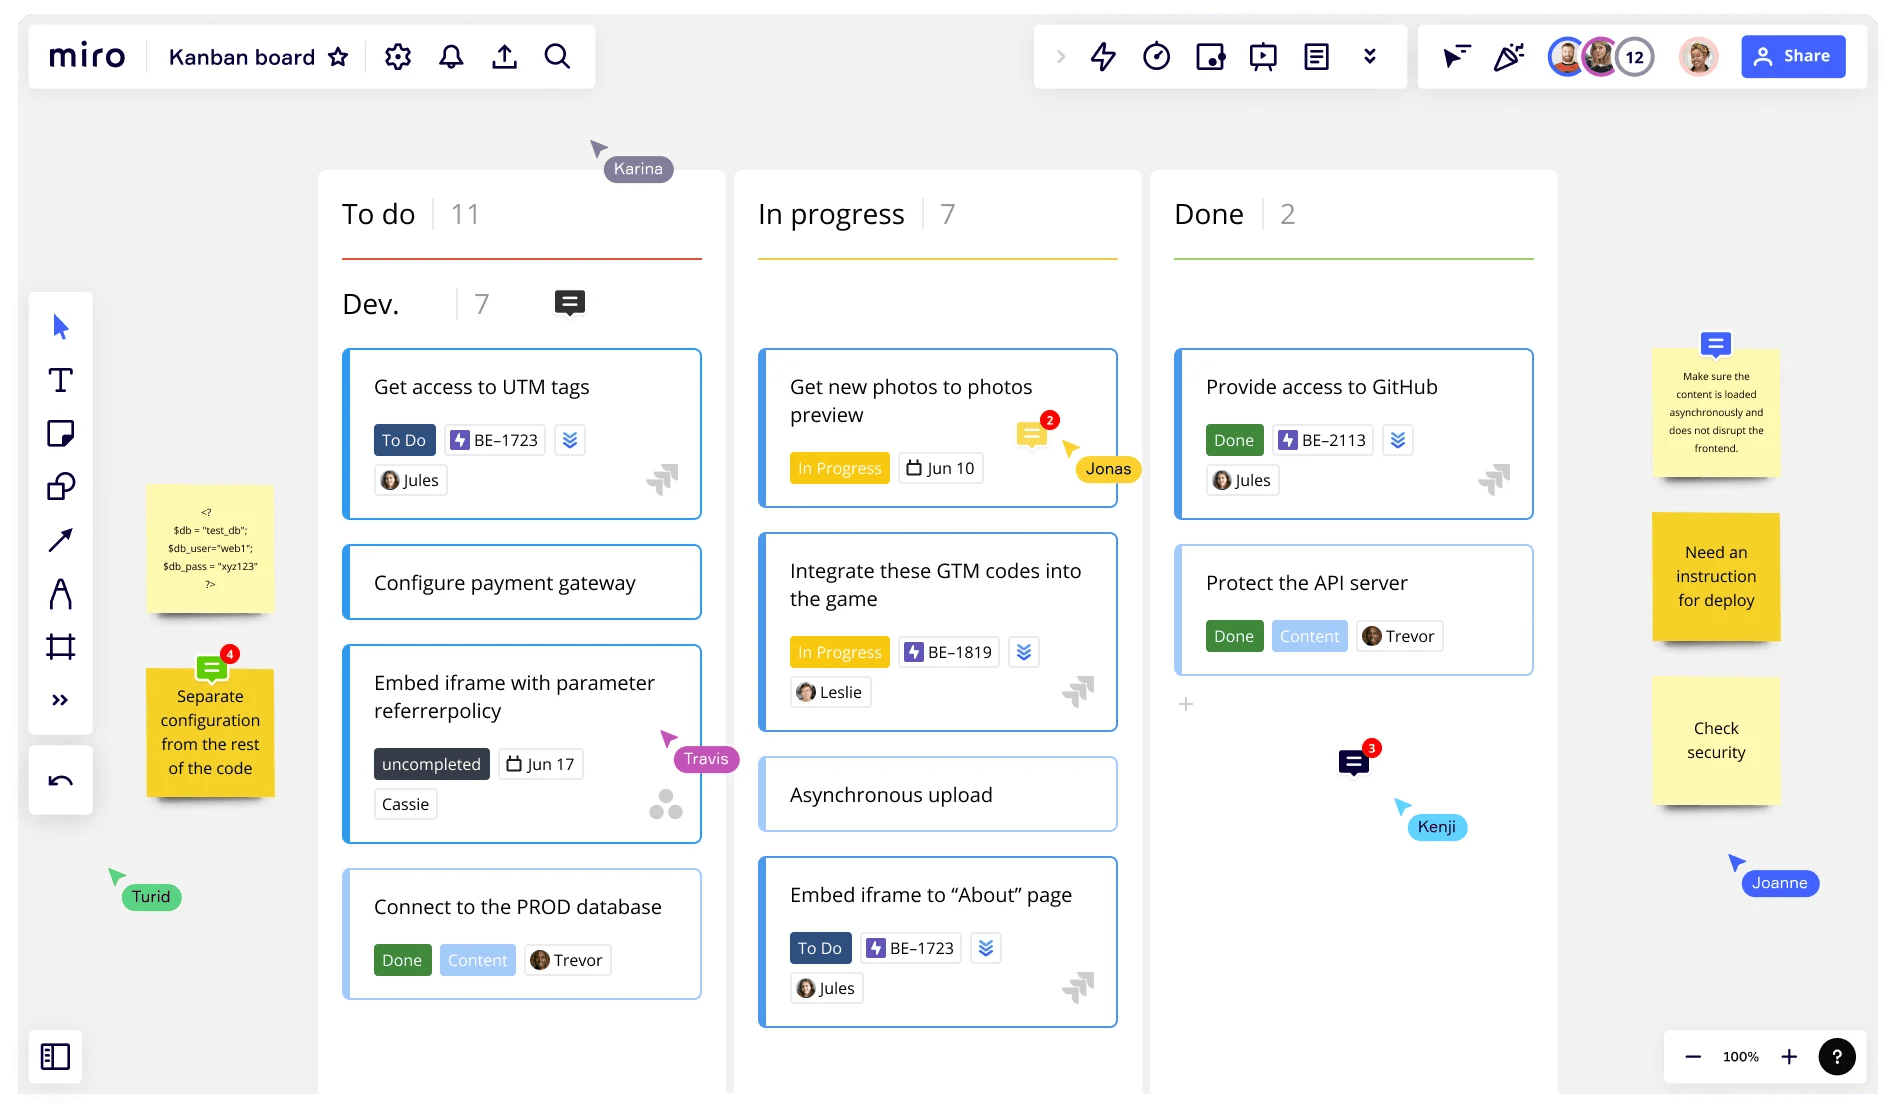
\includegraphics[width=0.9\textwidth]{images/kanban-ejemplo.png}
\caption{Ejemplo básico de tablero Kanban con columnas, tarjetas, WIP y swimlanes.}
\end{figure}

Este ejemplo ilustra cómo la representación visual del trabajo facilita el seguimiento, la colaboración y la mejora continua.

